% =====================================================================
%  Research Report  --  Gezhi
%  2026 AI for SDGs: Global Youth AI Future Innovation Competition
%  Macau Secondary School Division
%
%  Compile:  pdflatex ResearchReport_Gezhi.tex   (run twice, for hyperref)
%  English-only, as required by the competition rules.
%
%  !!  SEARCH FOR "TO BE COMPLETED" BEFORE SUBMITTING  !!
%  Every placeholder that needs the team's own data is printed in RED.
% =====================================================================
\documentclass[11pt,a4paper]{article}

\usepackage[T1]{fontenc}
\usepackage[utf8]{inputenc}
\usepackage{lmodern}
\usepackage[margin=2.0cm,top=1.9cm,bottom=1.9cm]{geometry}
\usepackage{booktabs}
\usepackage{tabularx}
\usepackage{array}
\usepackage{enumitem}
\usepackage{titlesec}
\usepackage{xcolor}
\usepackage{tikz}
\usepackage{microtype}
\usepackage{caption}
\usepackage{fancyhdr}
\usepackage[hidelinks]{hyperref}
\usepackage{xurl}          % allow URLs to break at any character
\emergencystretch=2.5em
\setlength{\parskip}{2pt}

% ---- placeholder macro: anything needing the team's own data ---------
\newcommand{\fillin}[1]{\textcolor{red}{\textbf{[TO BE COMPLETED:\,#1]}}}
\newcommand{\fillc}[1]{\textcolor{red}{\textbf{[#1]}}}   % compact, for tables
\newcolumntype{R}{>{\raggedright\arraybackslash}X}

\titleformat{\section}{\normalfont\large\bfseries}{\thesection.}{0.55em}{}
\titlespacing*{\section}{0pt}{10pt}{4pt}
\titleformat{\subsection}{\normalfont\normalsize\bfseries}{\thesubsection}{0.5em}{}
\titlespacing*{\subsection}{0pt}{7pt}{2pt}
\titleformat{\subsubsection}[runin]{\normalfont\bfseries}{}{0em}{}[\hspace{0.5em}]
\titlespacing*{\subsubsection}{0pt}{5pt}{0.5em}

\setlist[itemize]{leftmargin=1.2em,itemsep=1.5pt,topsep=2pt,parsep=0pt}
\setlist[enumerate]{leftmargin=1.5em,itemsep=1.5pt,topsep=2pt,parsep=0pt}
\setlength{\parskip}{3pt}
\setlength{\parindent}{0pt}
\captionsetup{font=small,labelfont=bf}

\pagestyle{fancy}
\fancyhf{}
\fancyhead[L]{\footnotesize \textsc{Gezhi} --- Research Report}
\fancyhead[R]{\footnotesize \thepage}
\renewcommand{\headrulewidth}{0.4pt}

\newcommand{\gezhi}{\textsc{Gezhi}}
\newcommand{\xiaoge}{\textsc{Xiaoge}}

\begin{document}

% ===================== TITLE ========================================
\begin{center}
{\LARGE\bfseries Gezhi: A Local-First AI Study Companion\\[3pt]
Built on Learning by Teaching}\\[7pt]
{\small 2026 AI for SDGs --- Global Youth AI Future Innovation Competition\\
Macau Secondary School Division \quad$\vert$\quad Theme: AI and Education}\\[4pt]
{\footnotesize
Team \textit{[Team Name]} \quad$\cdot$\quad \textit{[School Name]}\\[2pt]
\textit{[Student 1]}, \textit{[Student 2]}, \textit{[Student 3]}\\
Supervising teacher(s): \textit{[Teacher Name]}\\[2pt]
\today}
\end{center}
\vspace{-4pt}
\hrule
\vspace{6pt}

% ===================== ABSTRACT =====================================
\section*{Abstract}
\addcontentsline{toc}{section}{Abstract}

Two strands of evidence define the problem this project addresses. A randomised controlled
trial with roughly 1{,}000 secondary students found that unrestricted access to a large
language model improved practice performance by 48\% but \emph{reduced} examination
performance by 17\%; a carefully engineered hint-only tutor produced no examination benefit
at all. A separate two-year cluster randomised trial of an AI tutor across 18 middle schools
found effects of only 0.06--0.08 standard deviations, comparable to the same platform
without AI, because the median student used the tutor on just one third of practice days.
Together these results suggest that AI tutoring currently either harms learning or goes
unused, and that neither making the model more capable nor making it more careful addresses
the underlying cause.

\gezhi{} is a Windows desktop study companion for secondary-school students in Macau that
attacks both failure modes at once. It requires the student to \emph{produce} an explanation
rather than consume one, and it delivers that requirement proactively through a scheduling
system rather than waiting to be opened. The student teaches an on-screen companion,
\xiaoge{}, who is deliberately positioned a year below them and who holds a fixed library of
misconceptions drawn from the student's own error statistics. The companion argues back; it
concedes only when the explanation genuinely addresses the misconception. Explanations are
scored on a six-dimension rubric, and the resulting mastery estimate schedules both
questions and future explanations. Retrieval runs locally over the student's own textbook
using a trigram full-text index with page-level citations.

\textbf{Keywords:} AI in education; learning by teaching; teachable agents; retrieval
practice; metacognitive calibration; local-first software; SDG 4.

\vspace{4pt}
\hrule

% ===================== 1. BACKGROUND ================================
\section{Background}

\subsection{The promise and the first evidence}

Generative AI has been widely promoted as the technology that will finally deliver
one-to-one tutoring to every learner. The evidence accumulating since 2024 is considerably
more complicated, and it is worth stating precisely, because it shaped every design decision
in this project.

Bastani et al.\ (2024) conducted a randomised controlled trial with approximately 1{,}000
high-school students in Turkey learning mathematics, assigning them to three conditions:
business-as-usual practice, practice with unrestricted access to a general-purpose chatbot,
and practice with a version of the same model engineered to provide hints without revealing
answers. Students in the unrestricted condition solved 48\% more practice problems correctly
--- and then scored \textbf{17\% worse} on the examination once the AI was removed. Students
in the hint-only condition improved their practice performance by 127\%, but their
examination performance was statistically indistinguishable from the control group that
used no AI at all. The authors found that the model's step-by-step solutions were wrong 42\%
of the time, and that students overwhelmingly used it as a source of answers rather than as
a tutor.

A second study addresses a different failure mode. Oreopoulos and Low (2026) report a
two-year cluster randomised trial of Khanmigo, an AI tutor deliberately configured to coach
rather than answer, across 18 middle schools. The intent-to-treat effect was 0.06--0.08
standard deviations over a school year, with an implied effect of 0.14 SD for a full year of
active participation --- a range comparable to the same platform used \emph{without} AI
assistance. The authors are explicit about the cause, and it is behavioural rather than
technical: 96\% of students tried the tutor at least once, but the median student messaged it
on only one third of the days on which they practised, and in only \textbf{17\% of the
sessions in which they made a mistake}. Their conclusion is that ``realizing the promise of
AI tutoring will require getting students to use it, not just giving them access.''

\subsection{What the two results jointly imply}

Taken together, these findings carve out a narrow space in which an AI learning tool can
plausibly help:

\begin{enumerate}
  \item \textbf{Making the model answer better is not the solution.} The unrestricted
  condition answered most practice questions correctly and still harmed examination
  performance.
  \item \textbf{Making the model more restrained is also not sufficient.} The hint-only
  tutor was well designed and produced no examination gain.
  \item \textbf{The binding constraint is who produces the content.} The only condition that
  has never been shown to harm learning is the one in which the learner generates the
  explanation.
  \item \textbf{Delivery is as important as pedagogy.} An intervention that must be
  voluntarily opened will, empirically, not be opened.
\end{enumerate}

Points 3 and 4 are the design brief for \gezhi{}. The first is addressed by making
explanation, not consumption, the central act of the application. The second is addressed by
making explanations schedulable items in a spaced-repetition queue that surfaces on the
application's first screen.

\subsection{The local context}

Macau secondary students work from a mixture of Chinese-language and English-language
materials, frequently in scanned form, and face a high-stakes examination structure. Two
practical consequences shaped the system: full-text retrieval must work correctly on
Chinese text without a server, and scanned material must be ingestible. Both are addressed
in Section 5.2.

\subsection{Contribution}

This report describes (i) the design of a teachable-agent study companion for secondary
learners, in which deliberate and \emph{consistent} misconception is a first-class system
component; (ii) a local-first retrieval architecture that grounds the companion's challenges
in the student's own textbook; (iii) the coupling of explanation quality to a
spaced-repetition schedule; and (iv) an evaluation protocol and the results obtained with
secondary-school participants in Macau.

% ===================== 2. PROBLEM DEFINITION ========================
\section{Problem Definition}

\subsection{Research questions}

\begin{description}[leftmargin=1.4em,style=nextline,itemsep=3pt]
  \item[RQ1 --- Explanation quality.] Can a teachable companion that is engineered to hold
  consistent misconceptions, and that refuses to concede prematurely, improve the quality of
  a secondary student's spoken explanation of a knowledge point, as measured by a
  six-dimension rubric?
  \item[RQ2 --- Grounded challenge.] Can a fully local retrieval layer over the student's own
  textbook supply the companion with challenges that are specific enough to be useful and
  citable enough to be verifiable, without sending any content to a server?
  \item[RQ3 --- Proactive delivery.] Does scheduling \emph{explanations} --- not only
  questions --- in the review queue increase the frequency with which students actually
  explain, relative to an application in which explaining must be initiated manually?
  \item[RQ4 --- Calibration.] Does repeated teach-and-defend practice reduce the gap between
  a student's self-assessed understanding and their measured explanation quality?
\end{description}

\subsection{Target users and scope}

The primary user is a secondary-school student in Macau, aged approximately 14--18, studying
towards school examinations and university entrance. The design target is specifically the
student who believes they understand a topic but cannot articulate it --- a misjudgement
that is well documented. Across 115 studies, 15{,}889 participants and 502 effect sizes, the
weighted mean correlation between learners' judgements of their own learning and their
actual performance is only \(r = .178\) (Yang et al., 2022). The system is not designed for
primary-school children, nor for learners with no prior exposure to the material: several of
the techniques it relies upon require a knowledge base to operate on (Section 3.3).

\subsection{Non-goals}

\gezhi{} is not a homework-answering tool, does not generate answers to be copied, and does
not attempt to replace classroom instruction. It contains no social or competitive features,
by design: the application is single-user and local, and no student data is compared across
users or transmitted off the device.

% ===================== 3. RELATED WORK ==============================
\section{Related Work}

\subsection{Learning by teaching and teachable agents}

The pedagogical value of preparing to teach is long established. Chase, Chin, Oppezzo and
Schwartz (2009) demonstrated a \emph{protégé effect}: learners who believed they would teach
a virtual student invested more effort and achieved better outcomes than learners who
studied for themselves. That work, and the broader teachable-agent literature, established
the mechanism \gezhi{} relies on --- responsibility for another's understanding changes how
a learner processes material.

\subsection{LLM-based teachable agents, 2024--2026}

Recent work has moved this idea onto large language models, and has produced two findings
that directly shaped our design.

Yang, Pujara and Li (2025) inverted the standard tutor relationship, having students act as
instructors who must teach a model to solve problems. Their central design device is the
\emph{engineered knowledge gap}: questions constructed so that only the student holds the
information required to answer them. In an undergraduate course, this produced statistically
significant improvement over historical cohorts. The paper notes explicitly that a model
which answers too accurately removes the learning opportunity altogether.

Rogers et al.\ (2025), in work whose title --- ``Playing Dumb to Get Smart'' --- states the
design principle, created and evaluated an LLM-based teachable agent and found that the
agent must present itself as genuinely less capable for the interaction to be pedagogically
productive. A related study of a model used as a teachable agent in programming education
reported gains in knowledge and self-regulated learning but \textbf{no significant
improvement in error-correction ability}, for a specific and instructive reason: the model
tended to supply correct code directly, so students never got the opportunity to debug
anything.

That null result is the single most important piece of evidence for \xiaoge{}'s design. It
demonstrates that a teachable agent which is helpful in the ordinary sense is pedagogically
inert. The agent must be \emph{reliably and consistently wrong} in specific, diagnosable
ways.

\subsection{Established techniques, and what remains unaddressed}

To avoid rebuilding what already exists, we surveyed the current landscape of AI study
tools. The following are effectively commoditised: adaptive spaced-repetition scheduling
(with open-source algorithms now outperforming earlier fixed-interval methods on
large-scale benchmarks), knowledge-graph-driven question recommendation, Socratic dialogue
tutoring, and one-click conversion of source material into flashcards, quizzes or audio.
These are entry requirements rather than differentiators.

By contrast, three areas remain largely unaddressed in consumer products: role reversal, in
which the student teaches and the AI exposes its own misconceptions; deliberately designed
pretesting, in which the learner attempts a problem before instruction; and proactive,
evidence-driven delivery of the learning task at the moment it is needed. \gezhi{} is
positioned in the first and third of these.

We also adopted, with appropriate caution, techniques with strong but bounded evidence.
Interleaved practice has a moderate overall effect (\(g = 0.42\); Brunmair \& Richter, 2019)
and, uniquely among the techniques we considered, direct classroom evidence at secondary
level: in a three-month study with 126 seventh-grade students, interleaved practice produced
\(d = 0.42\) on an immediate test and \(d = 0.79\) on a test 30 days later (Rohrer, Dedrick
\& Stershic, 2014). The same meta-analysis reports that interleaving \emph{harmed} vocabulary
learning (\(g = -0.39\)), so \gezhi{} restricts interleaving to mathematics and science and
disables it for language vocabulary.

% ===================== 4. SYSTEM DESIGN =============================
\section{System Design}

\subsection{Architecture}

\gezhi{} is a single-user Windows desktop application. Its defining architectural property
is that the boundary of what the AI may touch is enforced by the operating system rather
than by instructions in a prompt.

\begin{figure}[h]
\centering
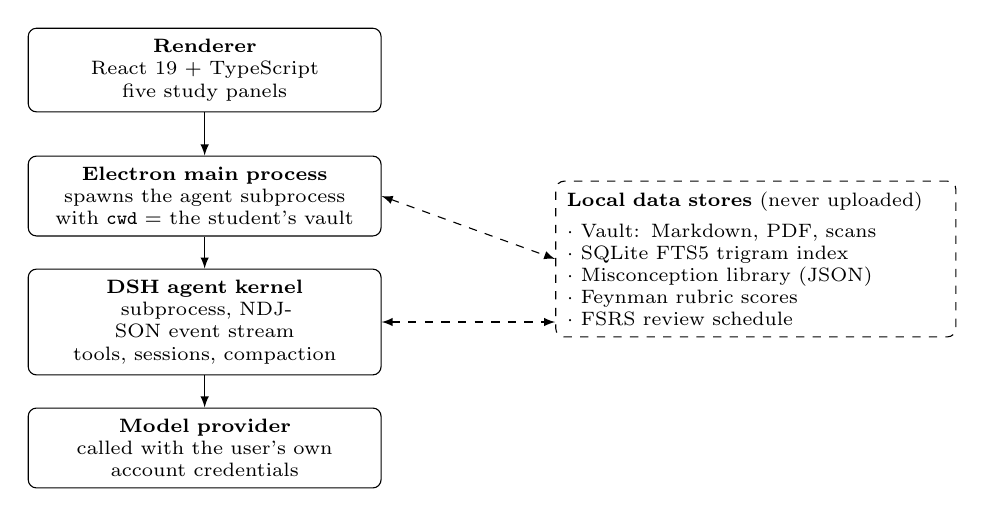
\begin{tikzpicture}[
  font=\scriptsize,
  >=latex,
  b/.style={draw,rounded corners=3pt,align=center,inner sep=4pt,minimum height=9mm},
  d/.style={draw,dashed,rounded corners=3pt,align=left,inner sep=4pt}
]
  \node[b,text width=42mm] (ui)   at (0,0)     {\textbf{Renderer}\\React 19 + TypeScript\\five study panels};
  \node[b,text width=42mm] (main) at (0,-1.6)  {\textbf{Electron main process}\\spawns the agent subprocess\\with \texttt{cwd} = the student's vault};
  \node[b,text width=42mm] (dsh)  at (0,-3.2)  {\textbf{DSH agent kernel}\\subprocess, NDJSON event stream\\tools, sessions, compaction};
  \node[b,text width=42mm] (llm)  at (0,-4.8)  {\textbf{Model provider}\\called with the user's own\\account credentials};

  \node[d,text width=48mm] (data) at (7.0,-2.4)
    {\textbf{Local data stores} (never uploaded)\\[3pt]
     $\cdot$ Vault: Markdown, PDF, scans\\
     $\cdot$ SQLite FTS5 trigram index\\
     $\cdot$ Misconception library (JSON)\\
     $\cdot$ Feynman rubric scores\\
     $\cdot$ FSRS review schedule};

  \draw[->] (ui)   -- (main);
  \draw[->] (main) -- (dsh);
  \draw[->] (dsh)  -- (llm);
  \draw[<->,dashed] (main.east) -- (data.west);
  \draw[<->,dashed] (dsh.east)  -- (data.west |- dsh.east);
\end{tikzpicture}
\caption{System architecture. The agent kernel runs as a separate process whose working
directory is the student's vault; its write boundary is derived from that directory, so it
cannot modify anything outside it. All retrieval, scoring and scheduling data remain on the
device.}
\label{fig:arch}
\end{figure}

\subsection{The learning loop}

The application is organised around a single recurring sequence, shown in Table~\ref{tab:loop}.
The ordering is deliberate: the student attempts the material before it is explained,
commits to a self-assessment before receiving feedback, produces the explanation themselves,
and is then challenged on it.

\begin{table}[h]
\centering
\small
\begin{tabularx}{\textwidth}{@{}c p{3.4cm} R@{}}
\toprule
\textbf{\#} & \textbf{Stage} & \textbf{What happens} \\
\midrule
0 & Trigger & The review queue surfaces a due knowledge point on the first screen. \\
1 & Pretest & The student attempts one item and may answer ``I don't know''. No feedback is given yet. \\
2 & Self-rating & The student rates their own understanding on a 1--5 scale. \\
3 & Explain & The student explains the topic aloud to \xiaoge{}. The companion does not interrupt. \\
4 & Challenge & \xiaoge{} raises one of its stored misconceptions and argues. The student must resolve it. \\
5 & Score & A six-dimension rubric scores the explanation against the textbook source. \\
6 & Repair & The system generates targeted items for the specific gaps identified. \\
7 & Schedule & Both questions and future explanations are scheduled by an FSRS-based model. \\
8 & Delayed self-rating & On a later day, the student re-rates their understanding \emph{after} attempting retrieval. \\
\bottomrule
\end{tabularx}
\caption{The \gezhi{} learning loop. Stages 1, 2 and 8 correspond to pretesting, immediate
calibration and delayed calibration respectively.}
\label{tab:loop}
\end{table}

\subsection{\xiaoge{}: engineering a reliably wrong companion}

The companion is not an assistant. It is positioned as a student one year below the user,
and its function is to make the user's explanation load-bearing.

Three properties are essential and each required explicit engineering:

\begin{itemize}
  \item \textbf{Stable identity.} The companion never evaluates, never says ``you are
  wrong'', and never compares the user to anyone.
  \item \textbf{Consistent misconceptions.} The companion's errors come from a structured
  library (Section 5.5), not from sampling noise. Consistency matters more than the errors
  themselves: if the companion's objection shifts each turn, the student learns that the
  system is unreliable rather than that they have a gap to close.
  \item \textbf{Hard refusal to concede prematurely.} Language models are strongly disposed
  to agree. The system prompt therefore imposes an explicit constraint: the companion may
  not signal understanding until the student's explanation satisfies the specific correction
  criterion attached to the active misconception. Without this constraint the interaction
  degenerates within two turns into dictation to a recording device.
\end{itemize}

The companion carries a three-by-three lattice above its head, which doubles as a progress
display: nine empty cells mean it understands nothing, and each resolved misconception
lights one cell in vermilion. This gives the student feedback on progress without presenting
a score, which is intended to keep the framing on teaching rather than on being graded.

% ===================== 5. TECHNICAL METHODS =========================
\section{Technical Methods}

\subsection{Agent kernel: subprocess isolation with an event stream}

Rather than implement an agent loop, \gezhi{} embeds DeepSeek Harness (DSH), an MIT-licensed
agent kernel, as a headless subprocess and consumes a newline-delimited JSON event stream.
Each event carries a type --- session, status, thinking, text, tool call, tool result,
final --- together with token accounting. This provides session persistence, a tool sandbox,
context compaction and an approval policy without requiring a student team to reimplement
them, and it keeps the model credential in the user's own account rather than in the
application.

The kernel derives its filesystem write boundary from its working directory, so launching it
with the working directory set to the student's vault produces a boundary enforced by the
process model. Two implementation details proved necessary in practice. First, the
subprocess must be started through its command wrapper rather than by invoking the host
executable directly, because the installation path contains spaces. Second, the event stream
must be decoded as UTF-8 explicitly; reading the redirected byte stream with a
non-UTF-8-aware reader corrupts Chinese content, and the corruption occurs on the reading
side only. A regression test that writes Chinese text and reads it back is part of the
build.

\subsection{Local retrieval: a measured tokeniser fix}

Retrieval is performed entirely on the device using SQLite, accessed through the runtime's
built-in module so that no native dependency is required. We measured behaviour rather than
assuming it, and found a failure that would have silently disabled retrieval for the primary
user population.

With the default \texttt{unicode61} tokeniser, a full-text index returns \textbf{zero}
results for Chinese substring queries, because the tokeniser treats an entire Chinese
sentence as one token. Switching the index to \texttt{tokenize='trigram'} resolves this.
Measured results over a 200-document corpus: Chinese queries return 0 hits under
\texttt{unicode61} and 200 hits in approximately 1\,ms under \texttt{trigram}, at a write
cost of roughly 20\% and a modest index size increase. Indexing the corpus of 200 documents
of 14{,}400 characters took 61\,ms and 73\,ms respectively.

Because the tokeniser is fixed at table-creation time, the schema is created once with
\texttt{trigram} and a migration path exists for databases created with the default. We
deliberately did not make vector search a precondition: keyword retrieval over a trigram
index is sufficient for the current corpus size, and adding an embedding dependency would
raise the installation cost on a student laptop.

\subsection{Citation-forced generation}

Every substantive claim the system presents must be traceable to a retrieved passage with a
page reference. The retrieval layer returns chunks of 300--500 characters with page
metadata, and the generation step is constrained to cite from those chunks. This serves two
purposes: it allows the student to verify the companion's challenge against their own
textbook, and it makes the companion's misconceptions diagnosable, since a student can see
which passage contradicts the objection.

\subsection{Explanation scoring}

Explanations are scored with a six-dimension rubric, returned as strictly structured JSON so
that scores persist and are comparable across sessions (Table~\ref{tab:rubric}). Each
dimension is scored 1--5. The rubric is applied against the retrieved textbook passage
rather than against the model's general knowledge, which keeps scores tied to the material
the student is actually being examined on.

\begin{table}[h]
\centering
\small
\begin{tabularx}{\textwidth}{@{}p{2.9cm} R@{}}
\toprule
\textbf{Dimension} & \textbf{What it measures} \\
\midrule
Accuracy & Whether the content of the explanation is correct with respect to the source. \\
Completeness & Whether all elements the source treats as required are present. \\
Causality & Whether the student explains \emph{why}, rather than restating \emph{what}. \\
Plain language & Whether the explanation avoids unexplained jargon. \\
Example quality & Whether a concrete, correctly chosen example is given. \\
Gap awareness & Whether the student flags what they are unsure about, rather than glossing over it. \\
\bottomrule
\end{tabularx}
\caption{The six-dimension explanation rubric. Scores are stored per knowledge point and
feed the review scheduler.}
\label{tab:rubric}
\end{table}

\subsection{Misconception library}

The companion's objections are drawn from a structured library rather than generated freely,
which is what makes them consistent and diagnosable. Each entry is stored as:

\begin{quote}
\ttfamily\small
\{ misconception\_id, surface\_claim, why\_wrong, correct\_point, trigger\_condition \}
\end{quote}

\texttt{surface\_claim} is the plausible but incorrect statement the companion will make;
\texttt{correct\_point} is the criterion the student's explanation must satisfy before the
companion concedes; \texttt{trigger\_condition} determines which knowledge points activate
the entry. An illustrative entry for English grammar: the surface claim ``\emph{must} and
\emph{may} both express possibility, so they can be used interchangeably,'' with the
correction that \emph{must} expresses near-certainty while \emph{may} expresses roughly
even likelihood.

Entries are derived from the student's own error statistics in the question bank, so the
misconceptions the companion holds are the ones the student actually makes.

\subsection{Interleaved practice generation}

The examination builder includes an interleaved mode that alternates knowledge points within
a single paper and, critically, does not label which topic each item belongs to ---
labelling removes the discriminative demand that produces the effect. Following the
meta-analytic finding that interleaving harms vocabulary acquisition, the mode is enabled
only for mathematics and science item types.

\subsection{Companion animation and speech}

The on-screen companion is implemented as a set of pre-rendered layers that are composed at
runtime --- body, head, eye states, brow states, five mouth shapes and the head lattice ---
rather than as frame-by-frame animation. Blinking, breathing and nodding are driven
procedurally. Mouth shapes are selected from the speech synthesiser's phoneme-level
timestamps, so lip synchronisation requires no audio analysis. The animation format is
animated WebP rather than GIF, because GIF's one-bit transparency produces visible edge
artefacts when the character is composited over the application interface.

Two behavioural rules reflect the pedagogical framing. First, expressions lag the content
rather than anticipate it: when the student makes an error, the companion first responds
with encouragement and only subsequently displays confusion, so that it reads as a peer
working through a problem rather than as an examiner. Second, the encouraging state is
triggered at least twice as often as the confused state.

\subsection{Examination typesetting}

The question bank exports typeset examination papers through XeLaTeX, which is required for
correct CJK typesetting. Where a system TeX distribution is present it is reused; where it
is absent the application falls back to printing through the embedded browser engine, so
that a missing TeX installation degrades the output quality rather than breaking the
feature.

% ===================== 6. DATA SOURCES ==============================
\section{Data Sources}

\gezhi{} ships with no textbook content. The knowledge base is populated by the student from
material they already possess, which is both a legal and a pedagogical decision: it removes
any question of redistributing copyrighted textbooks, and it ensures the companion's
objections concern the material the student is actually assessed on.

\begin{table}[h]
\centering
\small
\begin{tabularx}{\textwidth}{@{}p{4.4cm} p{3.6cm} R@{}}
\toprule
\textbf{Source} & \textbf{Type} & \textbf{Status and use} \\
\midrule
Student course textbooks and handouts & PDF, Word, Markdown & Supplied by the user; not redistributed. \\
Scanned worksheets and past papers & Image PDF & Ingested via OCR; OCR is a required path, not an optional one. \\
User's class notes & Markdown & Created inside the application. \\
Informatics knowledge-point outlines & Markdown & User-authored; imported as a knowledge-graph skeleton. \\
Publicly licensed question sets & Text & Imported only where the licence permits; recorded in an asset register. \\
\bottomrule
\end{tabularx}
\caption{Data sources. All material is user-supplied or explicitly licensed; no copyrighted
textbook content is bundled with the application.}
\label{tab:data}
\end{table}

\textbf{Licence discipline.} Dependencies are restricted to permissive licences (MIT, BSD,
Apache-2.0) suitable for a closed-source distribution. Components under AGPL were identified
during selection and excluded from the shipped product. Every external asset is recorded in
an asset register with its source URL and licence text.

% ===================== 7. TESTING ===================================
\section{Testing and Evaluation}

\subsection{Participants}

\fillin{number} secondary-school students from \fillin{school name}, Macau, in Secondary
\fillin{year levels}, aged \fillin{range}. Participation was voluntary and required written
consent from the student and a parent or guardian. \fillin{number} subject teachers
observed or reviewed the sessions.

\subsection{Procedure}

Each participant completed a single session of approximately \fillin{duration} minutes,
followed by a delayed session on the following day:

\begin{enumerate}
  \item \textbf{Pre-test} (5 items on the target knowledge point), followed by a self-rating
  of understanding on a 1--5 scale.
  \item \textbf{Teach-and-defend}, in which the participant explained the knowledge point
  aloud to \xiaoge{} and responded to its objections until either the misconception was
  resolved or a limit of \fillin{number} turns was reached.
  \item \textbf{Immediate rubric scoring} of the explanation.
  \item \textbf{Delayed session} (next day): a parallel form of the pre-test, followed by a
  second self-rating administered \emph{after} the retrieval attempt.
  \item \textbf{Short questionnaire} on perceived usefulness and perceived difficulty.
\end{enumerate}

\subsection{Measures}

\begin{table}[h]
\centering
\small
\begin{tabularx}{\textwidth}{@{}p{1.3cm} p{4.6cm} R@{}}
\toprule
& \textbf{Measure} & \textbf{Definition} \\
\midrule
M1 & Explanation quality & Total six-dimension rubric score (6--30) at stages 3 and 6 of the loop. \\
M2 & Immediate calibration gap & Absolute difference between self-rating (scaled to 30) and rubric total, at stage 2. \\
M3 & Delayed calibration gap & The same difference measured after the delayed retrieval attempt (stage 8). \\
M4 & Turns to resolution & Number of companion turns required to resolve the target misconception. \\
M5 & Delayed recall & Score on the parallel test form, administered one day later. \\
\bottomrule
\end{tabularx}
\caption{Evaluation measures. M2 and M3 follow the finding that delaying a judgement of
learning improves its relative accuracy substantially, while leaving overall optimism
largely unchanged.}
\label{tab:measures}
\end{table}

\subsection{Analysis}

Paired comparisons use Wilcoxon signed-rank tests given the expected sample size, with
matched-pairs rank-biserial correlation reported as an effect size. We report M5 as a
descriptive outcome rather than as an efficacy claim, and we caution against interpreting any
result from a single-arm design as causal (Section 9).

% ===================== 8. RESULTS ===================================
\section{Results}

\fillin{This entire section must be completed with the team's own measured data before
submission. Do not estimate, round up, or infer any value. If a measurement was not taken,
report it as not taken.}

\begin{table}[h]
\centering
\small
\begin{tabularx}{\textwidth}{@{}p{2.6cm} p{2.2cm} p{2.2cm} p{2.2cm} R@{}}
\toprule
\textbf{Measure} & \textbf{Pre} & \textbf{Post} & \textbf{Change} & \textbf{Test statistic} \\
\midrule
M1 Explanation quality & \fillc{mean $\pm$ SD} & \fillc{mean $\pm$ SD} & \fillc{value} & \fillc{statistic, $p$, effect size} \\
M2 Calibration gap (immediate) & --- & \fillc{value} & --- & --- \\
M3 Calibration gap (delayed) & --- & \fillc{value} & \fillc{vs M2} & \fillc{statistic, $p$} \\
M4 Turns to resolution & --- & \fillc{median (IQR)} & --- & --- \\
M5 Delayed recall & \fillc{value} & \fillc{value} & \fillc{value} & \fillc{statistic, $p$} \\
\bottomrule
\end{tabularx}
\caption{Results. \fillin{fill from the session logs exported by the application.}}
\label{tab:results}
\end{table}

\subsection{Qualitative observations}

\fillin{Two or three specific, quotable observations from the sessions. Useful examples:
a participant who changed their explanation after the third objection; a participant who
initially rated their understanding highly and revised it downward after failing the delayed
retrieval; any case where the companion's misconception was itself wrong and the student
correctly identified that. The last case is particularly valuable and should not be omitted.}

\subsection{Deviations from the protocol}

\fillin{Record honestly any session that did not follow the procedure --- missing data,
a participant who stopped early, a technical failure. Reporting these strengthens rather
than weakens the report.}

% ===================== 9. LIMITATIONS ===============================
\section{Limitations}

We state these plainly, because the evidence base described in Section 1 is precisely about
the danger of over-claiming.

\begin{itemize}
  \item \textbf{No control group.} The evaluation is single-arm, so improvements cannot be
  attributed to \gezhi{} rather than to practice, novelty, or the attention of being
  observed. Claims are limited to feasibility and to within-participant change.
  \item \textbf{Small sample, single site.} \fillin{n} participants at one school cannot
  support generalisation to Macau secondary education.
  \item \textbf{Short duration.} A single session with a one-day delayed test measures
  immediate retention, not durable learning. The spaced-repetition behaviour that the design
  depends on would require weeks to evaluate.
  \item \textbf{Self-report instruments.} Self-ratings of understanding are the object of
  study in M2 and M3 and are simultaneously self-reported, which is a confound we cannot
  remove within this design.
  \item \textbf{Model non-determinism.} The companion's objections vary between runs even
  with a fixed misconception library, because the surface wording is generated. This affects
  reproducibility of the interaction, though not of the underlying misconception.
  \item \textbf{Rubric validity.} The six-dimension rubric is our own construction. It has
  not been validated against external raters, and inter-rater reliability with human teachers
  has not yet been established.
  \item \textbf{Novelty is narrower than it may appear.} Teachable agents are an established
  research area, and 2024--2026 has produced several LLM-based systems of this kind. Our
  contribution concerns the population, the grounding of the challenge in the student's own
  material, the coupling to scheduling, and the local-first constraint --- not the invention
  of the mechanism.
\end{itemize}

% ===================== 10. ETHICS ===================================
\section{Ethics, Safety and Privacy}

\subsection{Data protection}

The knowledge base, the learning record and all scores reside on the student's device. No
student content is uploaded to a server operated by the team, and no analytics are collected.
Model inference is performed through the user's own account, and prompts are not retained by
the application. The agent kernel's write boundary is derived from the working directory at
process launch, so the AI cannot modify files outside the student's vault; this is enforced
by the operating system rather than by instruction.

Where a session requires network access, this is disclosed before the session begins. The
application degrades to local retrieval, local speech recognition and a text-only mode
rather than failing.

\subsection{Research with human participants}

Participation was voluntary. Informed consent was obtained in writing from each student and
from a parent or guardian, covering the purpose of the study, the data collected, and the
right to withdraw at any time without consequence. Participants were assigned codes; no
names, student numbers, faces or voices appear in any submitted material. Audio recordings
were used only for transcription during the session and were deleted afterwards. The study
was conducted with the knowledge and approval of the participating school.

\subsection{Responsible AI use and academic integrity}

Generative AI tools were used in this project for software development, for the analysis of
published research, and for the preparation of design assets. The complete disclosure is in
Appendix A. All reported data were produced by the student team through sessions they ran
themselves. No result in this report is generated, estimated or inferred by a model.
External research findings are cited to their original sources, and where a widely
circulating figure could not be verified against a primary source we have said so rather
than repeating it.

\subsection{Copyright}

No copyrighted textbook content is distributed with the application. The knowledge base is
built from material the user supplies. Third-party libraries are restricted to permissive
licences, and every external asset is recorded with its source and licence.

\subsection{Bias and safety}

Two risks were considered explicitly. First, the misconception library is drawn from the
student's own errors and therefore cannot introduce misconceptions the student does not
already hold; this limits the companion's ability to propagate novel incorrect content.
Second, the companion is instructed never to evaluate the student as a person, never to
compare them with others, and never to discourage. Encouragement is triggered more
frequently than confusion by design, so that the interaction reads as collaborative rather
than as assessment.

% ===================== 11. CONCLUSION ===============================
\section{Conclusion and Future Work}

\gezhi{} began from two findings that appear to leave no room for an AI learning tool: an AI
that answers questions harms examination performance, and an AI that does not answer
questions goes unused. Both failures share a cause --- the student is not the one producing
the content --- and that is the constraint the system is built around. The student explains;
an on-screen companion that is deliberately and consistently wrong makes that explanation
load-bearing; and the whole interaction is scheduled rather than left to the student's
initiative.

The immediate next steps are to complete a controlled comparison against a no-AI condition,
to validate the scoring rubric against human raters, and to run the evaluation over a period
long enough for the spaced-repetition schedule to matter. Beyond that, the most promising
extension is to make the companion's misconceptions visible to teachers as a class-level
picture of what students actually misunderstand --- which is information that current
assessment, focused on right and wrong answers, does not capture.

% ===================== REFERENCES ===================================
\begin{thebibliography}{99}
\small
\setlength{\itemsep}{1pt}
\setlength{\parsep}{0pt}

\bibitem{bastani2024} Bastani, H., Bastani, O., Sungu, A., Ge, H., Kabakci, O., \& Mariman,
R. (2024). \emph{Generative AI Can Harm Learning.} SSRN Working Paper.
\url{https://papers.ssrn.com/sol3/papers.cfm?abstract_id=4895486}

\bibitem{oreopoulos2026} Oreopoulos, P., \& Low, N. (2026). \emph{One Click Away: AI Tutoring
with Khanmigo in a Two-Year School Experiment.} NBER Working Paper 35620.
\url{https://doi.org/10.3386/w35620}

\bibitem{chase2009} Chase, C.~C., Chin, D.~B., Oppezzo, M., \& Schwartz, D.~L. (2009).
Teachable Agents and the Prot\'eg\'e Effect: Increasing the Effort Towards Learning.
\emph{Journal of Science Education and Technology, 18}(4).
\url{https://purl.stanford.edu/zm369yx3532}

\bibitem{yang2025} Yang, X., Pujara, H., \& Li, J. (2025). \emph{Learning by Teaching:
Engaging Students as Instructors of Large Language Models in Computer Science Education.}
COLM 2025. \url{https://arxiv.org/abs/2508.05979}

\bibitem{rogers2025} Rogers, et al. (2025). \emph{Playing Dumb to Get Smart: Creating and
Evaluating an LLM-based Teachable Agent within University Computer Science Classes.} CHI
2025. \url{https://doi.org/10.1145/3706598.3713644}

\bibitem{teachchatgpt2024} \emph{Learning by Teaching with ChatGPT: The Effect of Teachable
ChatGPT Agent on Programming Education.} arXiv:2412.15226.
\url{https://arxiv.org/abs/2412.15226}

\bibitem{dunlosky2013} Dunlosky, J., Rawson, K.~A., Marsh, E.~J., Nathan, M.~J., \&
Willingham, D.~T. (2013). Improving Students' Learning With Effective Learning Techniques.
\emph{Psychological Science in the Public Interest, 14}(1), 4--58.
\url{https://doi.org/10.1177/1529100612453266}

\bibitem{brunmair2019} Brunmair, M., \& Richter, T. (2019). Similarity Matters: A
Meta-Analysis of Interleaved Learning and Its Moderators. \emph{Psychological Bulletin.}
\url{https://doi.org/10.1037/bul0000209}

\bibitem{rohrer2014} Rohrer, D., Dedrick, R.~F., \& Stershic, S. (2014). Interleaved
Practice Improves Mathematics Learning. \emph{Journal of Educational Psychology.}
\url{https://doi.org/10.1037/edu0000001}

\bibitem{richland2009} Richland, L.~E., Kornell, N., \& Kao, L.~S. (2009). The Pretesting
Effect: Do Unsuccessful Retrieval Attempts Enhance Learning? \emph{Journal of Experimental
Psychology: Applied.} \url{https://doi.org/10.1037/a0016496}

\bibitem{yang2022} Yang, et al. (2022). Meta-analysis of the accuracy of judgements of
learning. \emph{Review of Educational Research.}
\url{https://doi.org/10.3102/00346543221094083}

\bibitem{rhodes2011} Rhodes, M.~G., \& Tauber, S.~K. (2011). The Influence of Delaying
Judgments of Learning on Metacognitive Accuracy: A Meta-Analytic Review. \emph{Psychological
Bulletin.} \url{https://doi.org/10.1037/a0021705}

\bibitem{bisra2018} Bisra, K., Liu, Q., Nesbit, J.~C., Salimi, F., \& Winne, P.~H. (2018).
Inducing Self-Explanation: A Meta-Analysis. \emph{Educational Psychology Review, 30}(3).
\url{https://doi.org/10.1007/s10648-018-9434-x}

\bibitem{fan2024} Fan, Y., Tang, L., et al. (2024). Beware of Metacognitive Laziness: Effects
of Generative Artificial Intelligence on Learning Motivation, Processes, and Performance.
\emph{British Journal of Educational Technology.}
\url{https://doi.org/10.1111/bjet.13544}

\bibitem{unesco2024} UNESCO (2024). \emph{AI Competency Framework for Students} (Miao, F.,
Shiohira, K., \& Lao, N.). \url{https://unesdoc.unesco.org/ark:/48223/pf0000391105_eng}

\bibitem{expertium} Expertium. \emph{SRS Benchmark: FSRS versus SM-2 on a large Anki
collection.} \url{https://expertium.github.io/Benchmark.html}

\end{thebibliography}

% ===================== APPENDIX =====================================
\appendix
\section{AI Tool Disclosure}

The competition rules require teams to state the generative AI tools used, their versions,
their purpose, and the parts completed by the students. This appendix is that statement.

\begin{table}[h]
\centering
\small
\begin{tabularx}{\textwidth}{@{}p{3.2cm} p{1.5cm} p{3.0cm} R@{}}
\toprule
\textbf{Tool} & \textbf{Version} & \textbf{Purpose} & \textbf{Completed by students} \\
\midrule
\fillc{tool name} & \fillc{version} & \fillc{purpose} & \fillc{what the team did themselves} \\
\fillc{tool name} & \fillc{version} & \fillc{purpose} & \fillc{what the team did themselves} \\
\fillc{tool name} & \fillc{version} & \fillc{purpose} & \fillc{what the team did themselves} \\
\bottomrule
\end{tabularx}
\caption{Generative AI tools used in this project. \fillin{Complete every row before
submission; this table is checked against the competition's academic integrity rules.}}
\label{tab:ai}
\end{table}

\textbf{Division of work.} The problem identification, the research design, the software
architecture, the misconception library, the evaluation sessions and the analysis of results
were carried out by the student team. Generative AI was used as a development assistant
(code generation and review, documentation) and as a research aid (locating and summarising
published literature, all of which was then read at source before citation). No reported
data were generated or estimated by an AI system.

\end{document}
